\chapter{Proposal of parallel approach}

TODO: popis kapitoli...a uvod co bude zahrnovat...

\section{Bottlenecks of current approach}
\label{05:bottlenecks}

If we remember the knowledge we acquired in Section \ref{02:sec:strimzisystemtests}, then one realises that the time required for a given test set is extremely time-consuming. It is easier to maintain the correctness of the program of the sequence computing model, but the benefit that parallelism offers is incomparable. Nevertheless, one has to ask oneself whether it is possible and whether it pays off. To answer such a question, we can use Amdahl's law, which we learned about in Section \ref{04:amdalhlaw}. For simplicity, assume that the unit of work will be a test case. It will therefore be necessary to map how many tests can be parallelised. We can find out by analysing whether it contains any shared variable against other tests. Once it does not contain any variable, we can declare the test as parallelisable. If a given test contains such a shared variable, it implies that such a test will have to run in an isolated environment. The manual analysis we performed found that 250 tests must be parallel, and 115 must be isolated. So if we apply Equation \eqref{eqn:einstein}, which we learned in Section \ref{04:amdalhlaw}. The total number of tests is 365. The parallelizable part is \emph{p = 250/365}. The sequence part will be equal to \emph{seq = 1 - p = 115/365}. For only four-core CPUs, we get the following acceleration \eqref{eqn:amdalhinpractice}.
\begin{equation}
    \label{eqn:amdalhinpractice}
    S = \frac{1}{1 - \frac{250}{365} + \frac{\frac{250}{365}}{\frac{4}{1}}} =\sim 2.1x \; acceleration
    \tag{3}
\end{equation}
If we increase the number of CPUs to 8, the total acceleration will be 2.5, and if we scale it to 16 CPUs, the acceleration will be almost 3x. Consequently, if we imagine that our system tests have a total executive time of 40 hours, all tests will last approximately 13 hours with parallelisation. Thus, with this first step, we just showed that it pays to parallelise.

Another disadvantage of the current approach is the non-use of multiple Namespaces. In our case, for each test suite, we always have one Namespace in which we operate. Parallelism allows us to manage multiple namespaces simultaneously while ensuring that the test cases do not overlap. Subsequently, we create in each Namespace Cluster Operator, again and again; this process usually takes one minute. The ideal approach should be that the Cluster Operator should see all Namespaces and must be shared for all test suites. Using this approach eliminates a lot of lost time. However, we must be aware of a particular test suite or the test case that will require a different Cluster Operator configuration. At that moment, we must guarantee that some label will annotate that single test case or the entire test suite to run in isolation.

The disadvantages of the current approach mentioned above may be clear arguments for why such a change is necessary. What is also necessary to mention is the structure of the Resources in the Strimzi system tests. These are classes that encapsulate both some pre-prepared templates and, at the same time, the whole mechanism of creation. 
\begin{figure}[!ht]
    \centering
    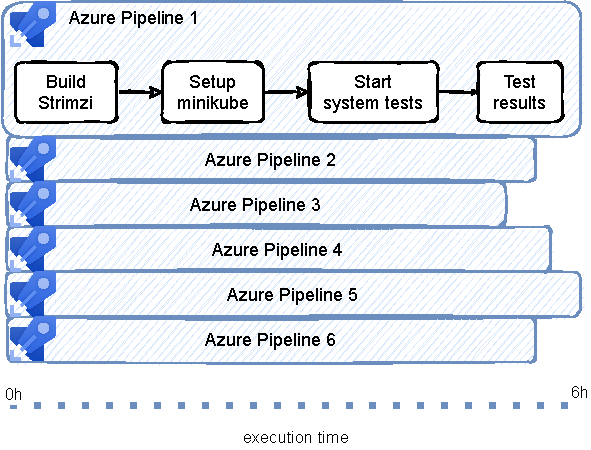
\includegraphics[scale=0.8]{obrazky-figures/06-proposal-of-parallel-approach/01a-azure_pipelines_with_test_results.pdf}
    \caption{Azure pipelines in form parallelism used to execute our system tests}
    \label{05:fig:azurepiplines}
\end{figure}
If we want to create a resource, we do it using \emph{KafkaResource.kafkaEphemeral(...).done()} and similarly with other resources. The correct API should propagate everything for the client writing the tests via the \emph{ResourceManager} class where a simple \emph{create()} method would be called. Nevertheless, this fact is more a matter of architecture and not a form of the execution model.

Finally, we can discuss the last limitation for which it is necessary to make a change. In the \ref{02:sec:strimzisystemtests} section, we did not mention such a fact, but there is an attempt of parallelism when using the Microsoft Azure Pipelines. On this infrastructure, we decompose our system tests into several distinctive subsets and run them as Azure separation pipelines \footnote{\textbf{Azure pipeline} \---\ one can imagine pipeline, as an Object which encapsulates multiple commands executed in order. Moreover, it is also executed as a separate process.}. In Figure \ref{05:fig:azurepiplines} one can see such decomposition. The attentive reader might realise why we cannot run such 40 or 100 Azure pipelines and thus eliminate the total execution time of the tests. Unfortunately, we are limited only to run six Azure Pipelines simultaneously. By this limitation, the total regression of the tests takes approximately 6 hours, which is not very satisfactory. Similarly, we try to reduce the time at the Jenkins pipeline when using the OpenStack and Amazon Web Services infrastructure. However, this Strimzi product must be verified for multiple configurations when running a Kubernetes separation cluster for the entire test suite. Once we launch several such Kubernetes clusters, we are also limited by infrastructure quotas. Overall execution time reduced can be seen in the following Figure \ref{05:fig:jenkinspipelines}. 
\begin{figure}[!ht]
    \centering
    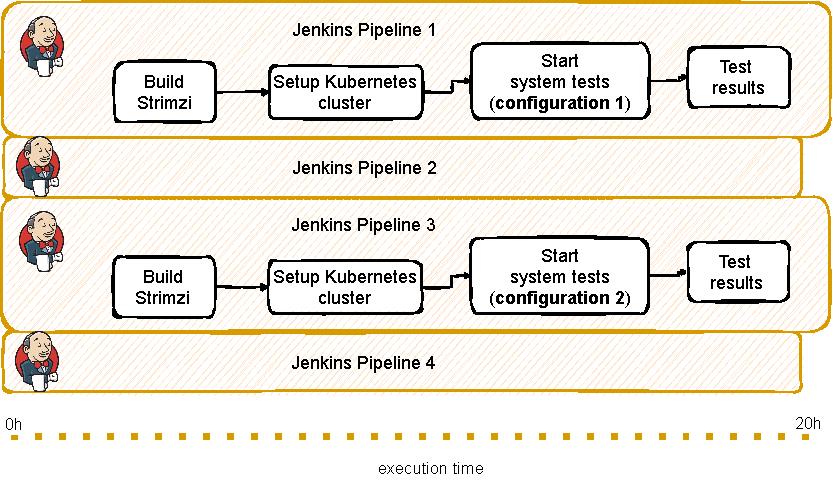
\includegraphics[scale=0.8]{obrazky-figures/06-proposal-of-parallel-approach/02-jenkins-smaller.pdf}
    \caption{Jenkins pipelines in a form parallelism used to execute our system tests}
    \label{05:fig:jenkinspipelines}
\end{figure}

What is also a duty to mention is that we are limited to the number of processes (i.e., pipelines) that always use the separation Kubernetes cluster. On Amazon Web Services and Openstack infrastructures, we are not limited to the computing resources we use. This is a fact that we must use and thus think about how parallelisation will lead the way. Undoubtedly, this will not be at the levels of processes, but parallelisation is possible directly in the test set (i.e., using threads) thanks to the available computational resources. However, this decision evokes the approaches described in the next section.

\section{Possible approaches}

From the previous section, we could notice that any attempt to parallelise at the process level (i.e., spawn more pipelines) was impossible, especially in terms of individual infrastructures' constraints. As a result, we have no choice but to go one level lower and try to parallelise at the test level and thus use the threads.

\subsection{Writing own testing framework}
\subsection{Writing own Junit5 Engine}
\subsection{JUnit5 paralelization}

\section{Architecture changes} % detection of conflicts, resourceManagerrework...bla bla
\section{Method wide paralelization}
\section{Class wide paralelization}
\section{Algorithms} 

\begin{algorithm}[H]
\label{01:alg:dsdsd}
\caption{Parallel algorithm for creation all resources inside \emph{Resource manager}}

\hspace*{\algorithmicindent} \textbf{Input: extensionContext, resources}

    \begin{algorithmic}[1]
        \ForEach{$resource \in resources$} 
            \State $type \gets findResourceType(resource)$
            \State $type.create(resource)$
            \\
            \State // here starts critical section
            \State $all\_resources.computeIfAbsent((test\_name), k -> new Stack<>())$
            \State $all\_resources.get((test\_name).push(deleteResource(resource)$
            \State // here ends critical section
            \\
        \If{wait for resource readiness}
            \ForEach{$resource \in resources$} 
                \State $type \gets findResourceType(resource)$
                \State wait for resource readiness
            \EndForEach
        \EndIf
        \EndForEach
    \end{algorithmic}
\end{algorithm}
